\begin{frame}
    \frametitle{Основные результаты работы}
    \small
    \begin{enumerate}
        \item \textbf{Модель:} интегрированный план выпуска, нарезки и расписания; лексикографическая целевая функция и десять технологических, временных и складских ограничений.
        \item \textbf{Численные методы:} полный перебор для малых задач и генетический поиск с конструктивным формированием планов, мутацией и парным отбором.
        \item \textbf{Имитационная модель:} оценка исполнения фиксированного плана при разбросе длительностей, отказах и ремонтах; показатели сроков, блокировок и загрузки ресурсов.
        \item \textbf{Комплекс и проверка:} реализация поиска и имитации; совпадение оценок $\mu$ с полным перебором на четырёх тестах; исследование плана на производственном экземпляре из $532$ рулонов.
    \end{enumerate}
\end{frame}
\note{
    Численные результаты сравнительной имитации нескольких планов в диссертации иллюстративны.
    Реализованный комплекс оценивает один план; достоверность реального сценария требует калибровки.
}

\begin{frame}
    \frametitle{Соответствие специальности 1.2.2}
    \small
    \begin{itemize}
        \item \textbf{п.~1:} математическая модель трёхкомпонентного производственного плана.
        \item \textbf{п.~2:} полный перебор и генетический поиск.
        \item \textbf{п.~3:} программная реализация численных методов.
        \item \textbf{п.~6:} дискретно-событийная модель исполнения расписания.
        \item \textbf{п.~8:} интегрированная постановка и вычислительное исследование.
        \item \textbf{п.~9:} численные эксперименты на тестовых и производственных данных.
    \end{itemize}
\end{frame}

\begin{frame}
    \frametitle{Научная новизна}
    \begin{enumerate}
        \item Разработана математическая модель совместного формирования и~оптимизации производственных планов и~расписаний в~целлюлозно-бумажной промышленности, в~которой решение представлено в~виде глобального плана $G=(\overline{\overline{X}},\overline{\overline{Y}},\overline{\overline{Z}})$, объединяющего план выпуска тамбуров, план раскроя и~расписание
        \item Предложена модель согласования стадий выпуска и~резки через~расписание и~динамику складов $(\overline{T},\overline{\overline{T}})$ с~учётом доступности полуфабрикатов, сроков и~размещения взаимодействующего оборудования в~одном цехе
        \item Разработан генетический поиск в~пространстве допустимых глобальных планов: изменение раскроя сопровождается пересчётом плана выпуска и~расписания
        \item Разработана дискретно-событийная модель исполнения расписания при случайных отклонениях длительностей, отказах и ремонтах оборудования
    \end{enumerate}
\end{frame}
\note{
    Научная новизна включает интегрированную модель плана,
    согласование выпуска и резки по расписанию с контролем складов,
    генетический поиск с пересчётом связанных компонент плана и
    дискретно-событийную модель исполнения при случайных возмущениях.
}

\begin{frame}
    \frametitle{Научная новизна}

\centering
\scriptsize
\resizebox{\textwidth}{!}{%
\begin{tabular}{|p{0.24\linewidth}|c|c|c|c|c|c|}
\hline
\textbf{Элемент постановки} &
\textbf{\shortstack{Воро-\\нов\\(2004)}} &
\textbf{\shortstack{Ур-\\бан\\(2015)}} &
\textbf{\shortstack{Леан,\\Толедо\\(2016)}} &
\textbf{\shortstack{Чен\\и~др.\\(2019)}} &
\textbf{\shortstack{Суджи-\\анто,\\Ян (2022)}} &
\textbf{\shortstack{Наст.\\работа}} \\
\hline
Генерация столбцов / ЛП & $+$ & $+$ & $+$ & $+$ & $-$ & $-$ \\
\hline
Метаэвристика & $-$ & $-$ & $-$ & $-$ & $+$ & $\boldsymbol{+}$ \\
\hline
Распределение заказов между БДМ & $+$ & $+$ & $+$ & $-$ & $-$ & $\boldsymbol{+}$ \\
\hline
Календарное планирование & $+$ & $+$ & $+$ & $-$ & $-$ & $\boldsymbol{+}$ \\
\hline
Учёт марок и плотности & $+$ & $+$ & $+$ & $-$ & $-$ & $\boldsymbol{+}$ \\
\hline
Несколько БДМ & $+$ & $+$ & $+$ & $-$ & $-$ & $\boldsymbol{+}$ \\
\hline
Многокритериальная ЦФ & $+$ & $+$ & $-$ & $-$ & $+$ & $\boldsymbol{+}$ \\
\hline
Программный комплекс & $+$ & $+$ & $-$ & $-$ & $-$ & $\boldsymbol{+}$ \\
\hline
Минимизация перестановок ножей & $+$ & $+$ & $-$ & $-$ & $-$ & $\boldsymbol{+}$ \\
\hline
\textbf{Многослойные заказы} & $-$ & $-$ & $-$ & $-$ & $-$ & $\boldsymbol{+}$ \\
\hline
\textbf{Максимум числа раскроев на ПРС} & $-$ & $-$ & $-$ & $-$ & $-$ & $\boldsymbol{+}$ \\
\hline
\textbf{БРС} & $-$ & $-$ & $-$ & $-$ & $-$ & $\boldsymbol{+}$ \\
\hline
\textbf{Динамика складов} & $-$ & $-$ & $-$ & $-$ & $-$ & $\boldsymbol{+}$ \\
\hline
\end{tabular}%
}

\end{frame}



\begin{frame}
    \frametitle{Практическая значимость}
    \begin{itemize}
        \item Комплекс формирует согласованные планы выпуска, раскроя и~расписания с~контролем производственных ограничений
        \item Имитационная модель позволяет оценивать чувствительность плана к~отклонениям длительностей и~отказам оборудования
        \item Результаты внедрены в деятельность ООО~«Опти-Софт»; имеется акт о внедрении
        \item Зарегистрированы программы для ЭВМ \textnumero\,2024611544 (23.01.2024) и~\textnumero\,2026618647 (26.03.2026)
    \end{itemize}
\end{frame}
\note{
    Практическая значимость: внедрение в ООО~«Опти-Софт», две регистрации программ для ЭВМ, возможность имитационной оценки построенного плана.
}

\begin{frame}
   \frametitle{Свидетельства о регистрации программ}
   \begin{figure}[h]
       \centering
       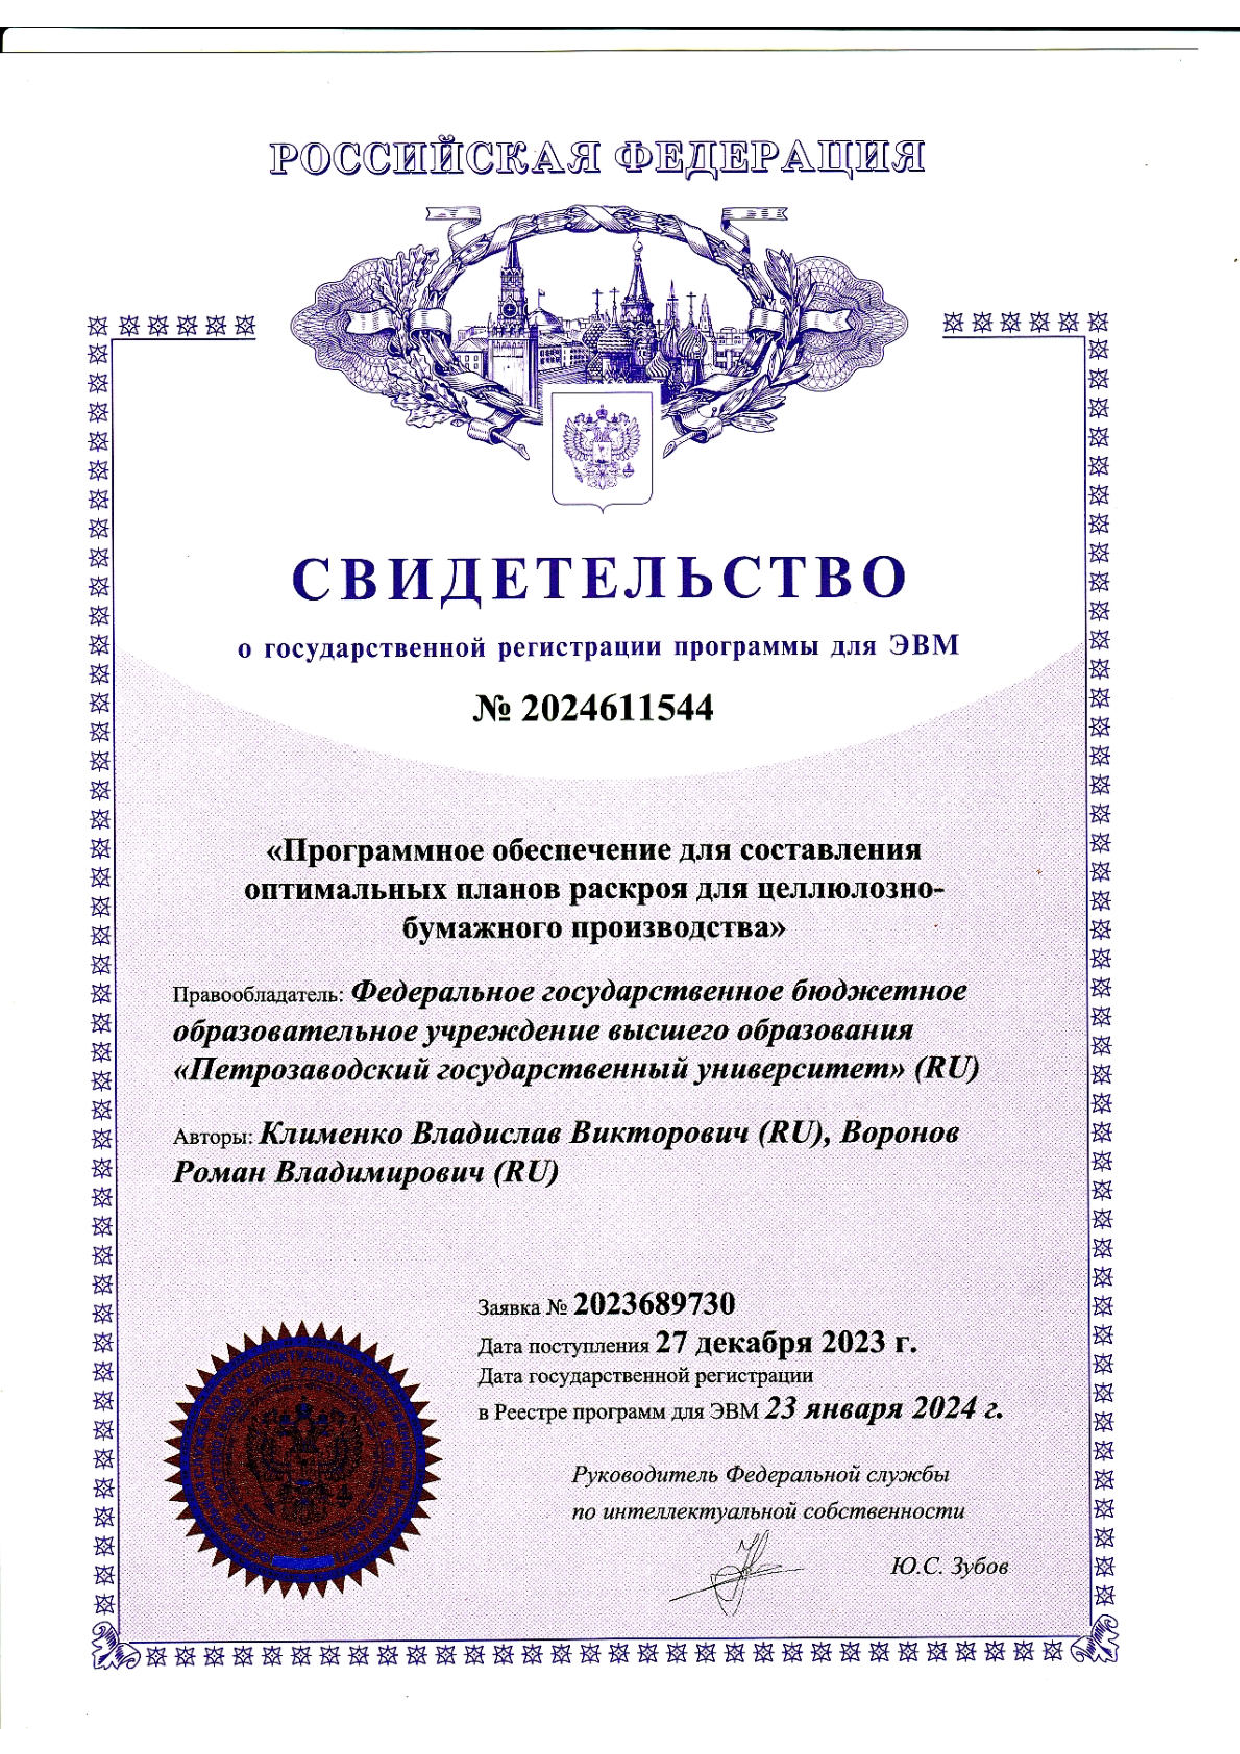
\includegraphics[height=0.7\textheight]{images/2024611544_program_registration}
       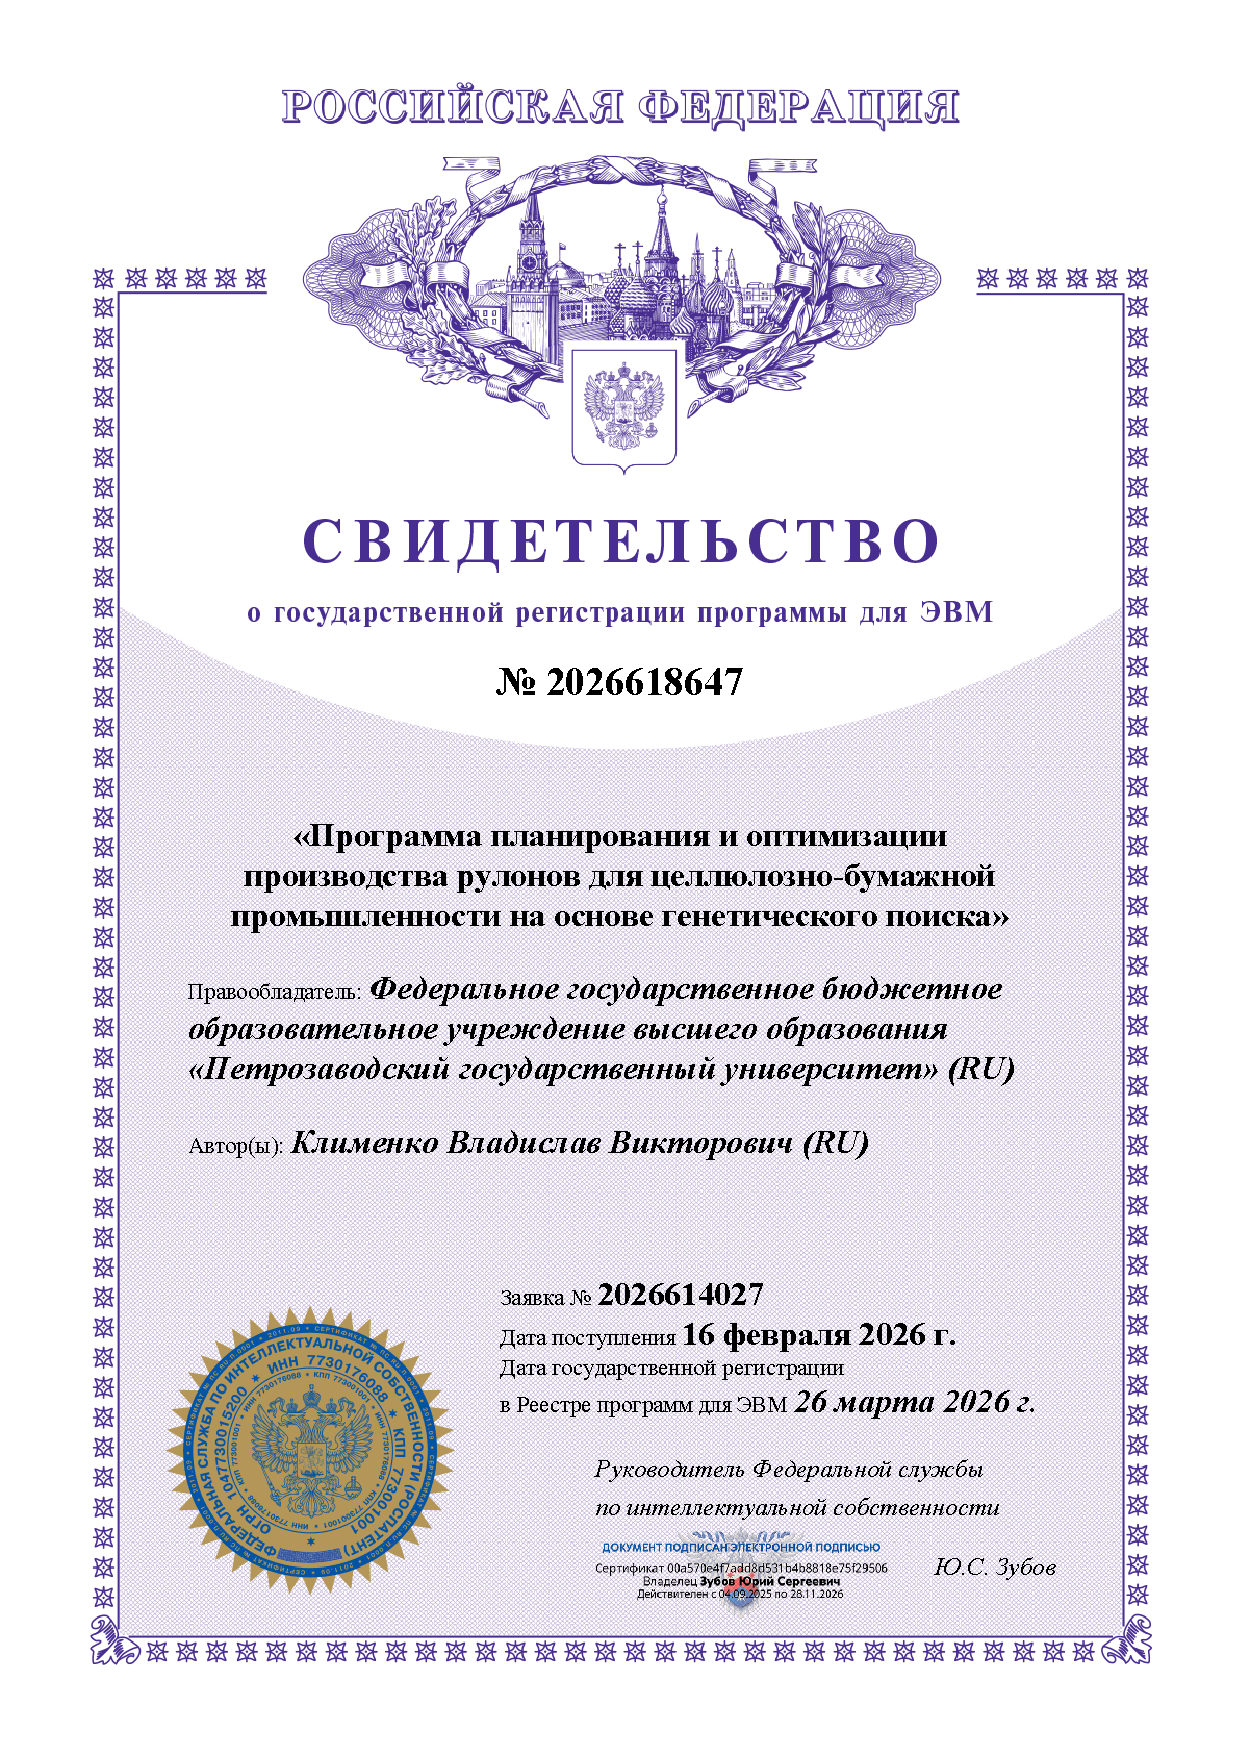
\includegraphics[height=0.7\textheight]{images/2026618647_program_registration}
   \end{figure}
\end{frame}
\note{
   Зарегистрированы две программы для ЭВМ: \textnumero\,2024611544 и \textnumero\,2026618647.
}

\begin{frame}
   \frametitle{Акт о внедрении}
   \begin{figure}[h]
       \centering
       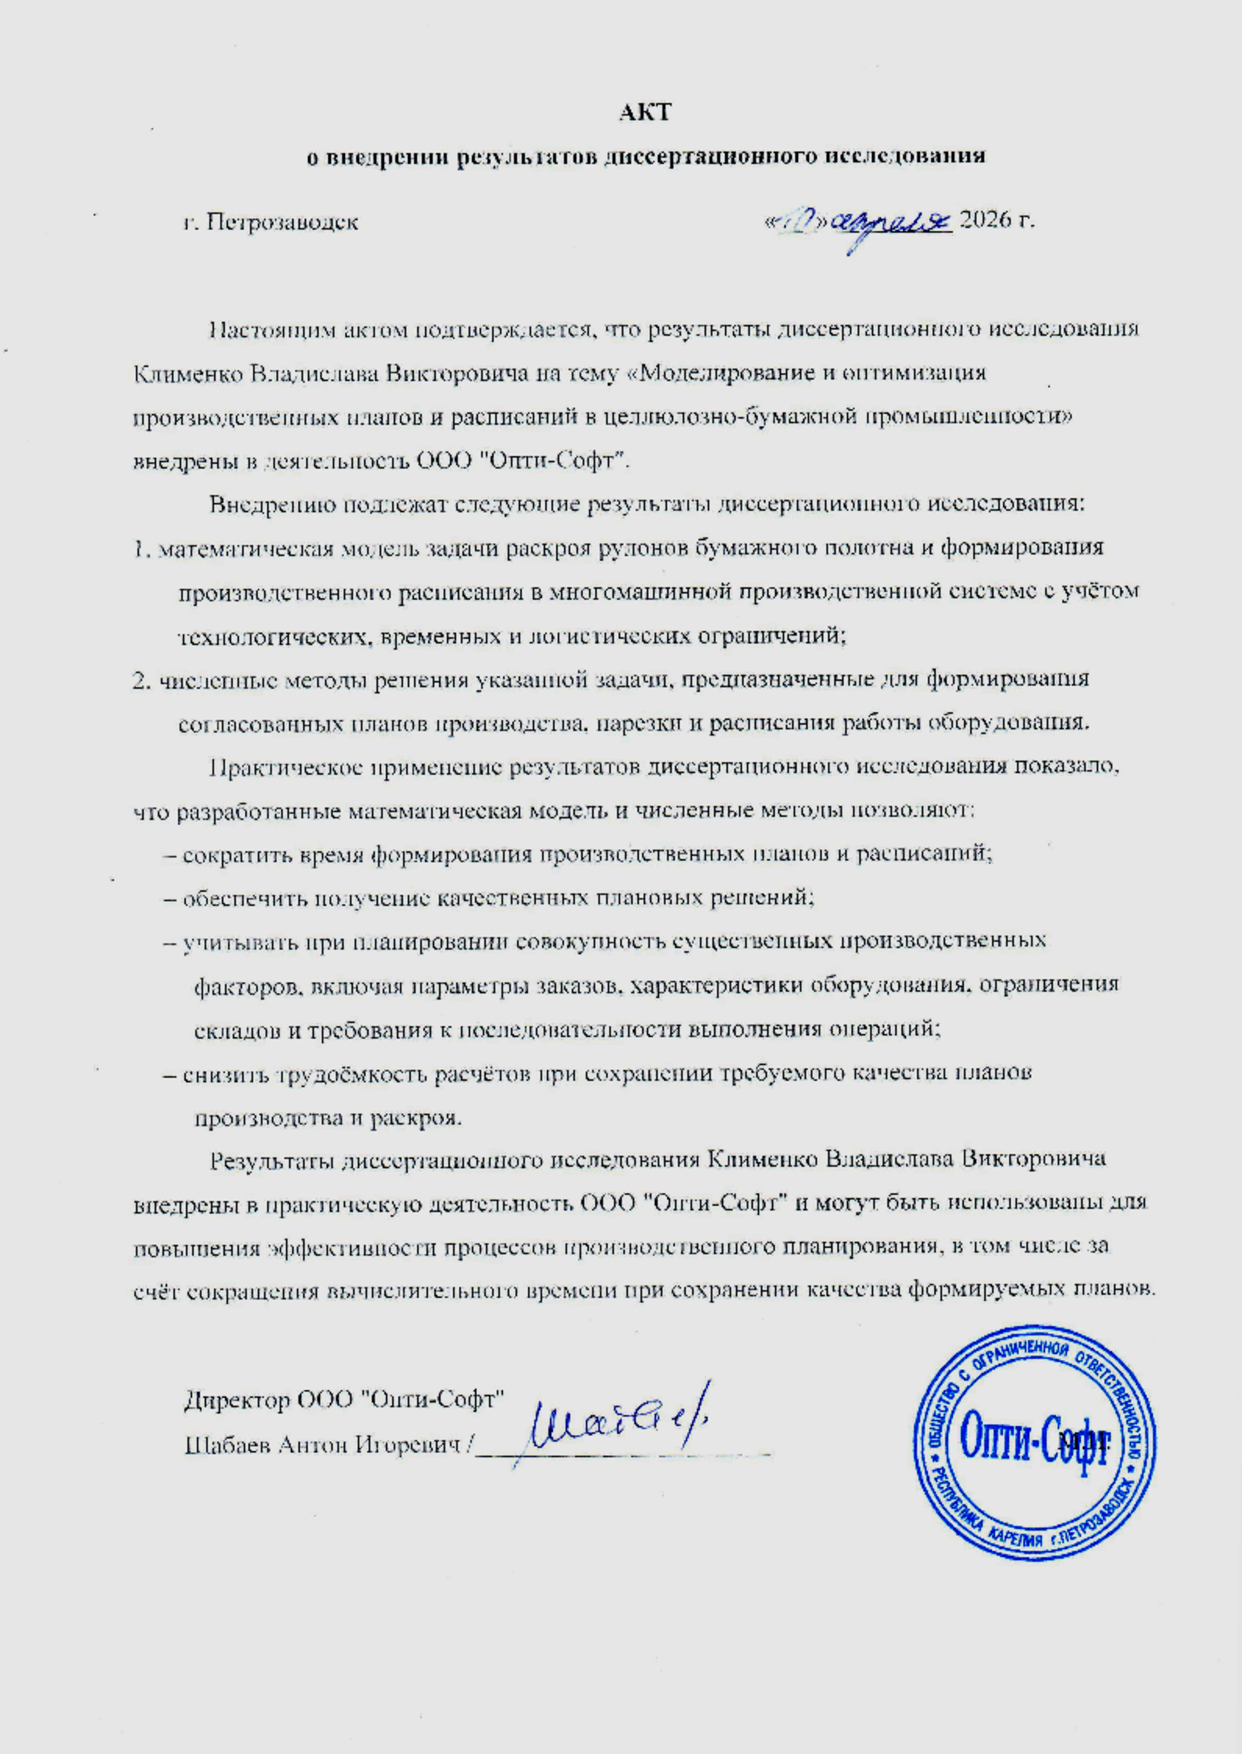
\includegraphics[height=0.85\textheight]{images/implementation.pdf}
   \end{figure}
\end{frame}
\note{
   Получен акт о внедрении.
}


\begin{frame}
    % \begin{frame}[t,allowframebreaks] % публикации на нескольких страницах
    \frametitle{Основные публикации}
    %% authorvak
    \nocite{klimenko2024_prin}%
    \nocite{klimenko2025ivdon}%
    \nocite{klimenko2026ubs}%
    %
    %% authorwos
    %\nocite{wosbib1}% TODO: заменить на реальный ключ публикации WoS, если появится
    %
    %% authorscopus
    \nocite{klimenko2025fruct}%
    %
    %% authorprogram
    % \nocite{Voronov_Klimenko_2024_patent}%
    
    \ifnumequal{\value{bibliosel}}{0}{
        \insertbiblioauthor
    }{
        \textbf{ВАК:}\printbibliography[keyword=biblioauthorvak,resetnumbers=true]%
        \textbf{Scopus:}\printbibliography[keyword=biblioauthorscopus,resetnumbers=true]%
    }
\end{frame}
\note{
    Согласно общей характеристике работы: 8 печатных публикаций,
    из них 3 публикации в журналах ВАК, 1 публикация в журнале,
    индексируемом международными базами, и 4 публикации в материалах конференций.
    Зарегистрированы 2 программы для ЭВМ.
}


\begin{frame}[t,allowframebreaks] % публикации на нескольких страницах
    \frametitle{Публикации РИНЦ}
    %% authorconf
    \nocite{klimenko2024moscow}%
    \nocite{klimenko2025itptz}%
    \nocite{klimenko2026vtp}%
    \nocite{klimenko2026review}

    
    \ifnumequal{\value{bibliosel}}{0}{
        \insertbiblioauthor
    }{
        \printbibliography[keyword=biblioauthorother,resetnumbers=true]%
    }
\end{frame}
\note{
    Согласно общей характеристике работы: 8 печатных публикаций,
    из них 3 публикации в журналах ВАК, 1 публикация в журнале,
    индексируемом международными базами, и 4 публикации в материалах конференций.
    Зарегистрированы 2 программы для ЭВМ.
}

\begin{frame}[t,allowframebreaks] % участия в конференциях
    \frametitle{Доклады на конференциях}
    \begin{enumerate}
        \item IV международная научно-практическая конференция «Современные исследования: теория, практика, результаты» (Москва, 15~февраля 2024~года)
        \item 76-я Всероссийская научная конференция обучающихся и молодых учёных с международным участием (Петрозаводск, 1--21~апреля 2024~года)
        \item 37-я конференция Open Innovations Association FRUCT (Хельсинки, 14--16~мая 2025~года)
        \item XIX Всероссийская научно-практическая конференция «Цифровые технологии в образовании, науке, обществе» (Петрозаводск, 9--12~декабря 2025~года)
        \item IV Всероссийская молодёжная научная конференция «Информационные технологии в высокотехнологичных производствах» (Санкт-Петербург, 12--13~марта 2026~года)
        \item Международная научно-практическая конференция «Теория и практика применения вычислительных и информационных технологий в отраслевых системах» (13--14~марта 2026~года)
    \end{enumerate}
\end{frame}
\note{
    Очные и заочные выступления
}

\begin{frame}[plain, noframenumbering] % последний слайд без оформления
    \begin{center}
        \Huge
        Спасибо за внимание!
    \end{center}
\end{frame}
